% V1.0 @2022-03-02
% V1.1 @2022-03-06

% 编译需要大约15秒

\documentclass{beamer}

\mode<presentation>
{
	\usetheme{CambridgeUS} %https://hartwork.org/beamer-theme-matrix/
	\usecolortheme{default}
	\usefonttheme{serif}  % or try default,serif, structurebold, ...
	% \setbeamertemplate{navigation symbols}{} % 右下角按钮
	\setbeamertemplate{caption}[numbered]
} 

%导言区导包
\usepackage{graphicx} %在导言区导入宏包
\usepackage{booktabs}
\usepackage{multirow} %EXCEL导出latex表格,需要这个包 
\usepackage{caption}
\usepackage{hyperref} %加入超链接
\usepackage{array} %为了居中
\newcolumntype{C}[1]{>{\centering\arraybackslash}m{#1}}
\usepackage{threeparttable} %表格尾注
\usepackage{amssymb} %为了surd

\usepackage{color} %文字颜色
\usepackage[english]{babel}
\usepackage[utf8x]{inputenc}
\usepackage[UTF8, scheme = plain]{ctex} % Menu里的compiler要改成XeLaTeX。



% 标题在导言部分设置
\title[ARMA-GARCH]{\large{基于ARMA-GARCH族模型的中国股票市场波动率分析}}
\subtitle{毕业论文中期汇报}
\author[``Qiuyi HUANG'']{黄秋逸}
\institute[SUSTech]{南方科技大学}
\date{Mar. 6 2022}
% \logo{\includegraphics[height=.7cm]{fig/sus-logo.png}} % 每一页都会有


\begin{document} %导言区结束

% 导入标题
\begin{frame}
  \titlepage
\end{frame}

% 导入目录
% \begin{frame}{Outline}
%   \tableofcontents
% \end{frame}

% 在开头与每个小节导入带强调的目录, 需要编译两遍!
% 目录以 Section &  Subsection 指出
\AtBeginSection[]
{
  \begin{frame}
    \frametitle{Table of Contents}
    \tableofcontents[currentsection]
  \end{frame}
}


% Part 1
\section{Timeline}
\begin{frame}{Timeline}
  \begin{figure}[htp]
    \centering
    \includegraphics[width = 12cm]{fig/timeline.jpg}
    \caption{Research timeline}
    % \label{fig:galaxy}
  \end{figure}
\end{frame}


% Part 2
\section{Objective}
\begin{frame}{Objective}
  Our objective is to introduce an ARMA-GARCH family model under six different innovation distribution assumptions. We will apply two different methods to perform the model selection and compare the results between them. The model is used to estimate the conditional variances of the Chinese stock market. The ARCH effect is found to be significant and this model shows some shared manner between two Chinese major stock indexs.
\end{frame}


% Part 3
\section{Prerequisites}
\subsection{ARMA Model}
\begin{frame}{ACF \& PACF}
  Let's begin with some basic definitions in the time series analysis.
  \begin{block}{Autocorrelation Function}
    Consider a time series $\{r_t\}$, the correlation function of $r_t$ and its past values $r_{t-\ell}$ is generalized as autocorrelation function at lag $\ell$:
    \begin{displaymath}
      \rho_{\ell}=\frac{\operatorname{Cov}\left(r_{t}, r_{t-\ell}\right)}{\sqrt{\operatorname{Var}\left(r_{t}\right) \operatorname{Var}\left(r_{t-\ell}\right)}}
    \end{displaymath}
  \end{block}

  \begin{block}{Partial autocorrelation function}
    Further, the correlation between $r_t$ and its past value $r_{t-l}$ after removing the effect of the intervening variables $r_{t-1} \cdots r_{t-l+1}$ is of interest. This coefficient is called the partial autocorrelation at lag l:
    \begin{displaymath}
      \begin{array}{c}
        \phi_{\ell \ell}=\operatorname{Corr}\left(r_{t}, r_{t-\ell} \mid r_{t-1} \cdots r_{t-\ell + 1} \right)
      \end{array}
    \end{displaymath}
  \end{block}

\end{frame}


\begin{frame}{ARMA Model}
  \begin{block}{AR(p) Model}
    \begin{displaymath}
      r_{t}=\phi_{0}+\phi_{1}
      r_{t-1}+\cdots+\phi_{p}
      r_{t-p}+\varepsilon_{t}
    \end{displaymath}
    where p is a non-negative integer and $\{\varepsilon_{t}\}$ is assumed to be a white noise series with mean zero and constant variance. This model says that the past p values $r_{t-i},~ i=1,2, \cdots ,p$ jointly determine the conditional expectation of ${r_{t}}$ given the past data.
  \end{block}

  \begin{block}{MA(q) Model}
    \begin{displaymath}
      r_{t}=c_{0}+\varepsilon_{t}-\theta_{1} \varepsilon_{t-1}-\cdots-\theta_{q} \varepsilon_{t-q}
    \end{displaymath}
    where q is a non-negative integer and $\{\varepsilon_{t}\}$ is assumed to be a white noise series with mean zero and constant variance.
  \end{block}
\end{frame}


\begin{frame}{ARMA Model}
  \begin{block}{ARMA(p,q) Model}
    \begin{displaymath}
      r_{t} =  \phi_{0}+\sum_{i=1}^{p} \phi_{i} r_{t-i}+\varepsilon_{t}-\sum_{i=1}^{q} \theta_{i} \varepsilon_{t-i}
    \end{displaymath}
    which is:
    \begin{displaymath}
    \left(1-\phi_{1} B^{1}-\cdots-\phi_{p} B^{p}\right) r_{t}=\phi_{0}+\left(1-\theta_{1} B^{1}-\cdots-\theta_{q} B^{q}\right) \varepsilon_{t}
    \end{displaymath}
    where ${\varepsilon_{t}}$ is a white noise series and p and q are non-negative integers. Backshift notation $B$ ensures $B*r_{t} = r_{t-1}$.
  \end{block}

  \begin{itemize}
    \item The AR(p) and MA(q) models are special cases of the ARMA(p, q) model. 
    \item The roots of $1-\phi_{1} x^{1}-\cdots-\phi_{p}x^{p}=0$ should lies out of the unit circle.
  \end{itemize}
\end{frame}


\subsection{Order Determination of ARMA Model}
\begin{frame}{ARMA Model Order Determination}
  \begin{itemize}
    \item We specify the order of AR and MA by ACF and PACF:
      \begin{tabular}{c c c c}
        \\ % 表格要换一行才好看
          \toprule[2pt]
          Model & AR(p) & MA(q) & ARMA(p,q)  \\ \midrule[1pt]
          ACF   & Not cut off   & Cut off at lag q &  Not cut off\\
          PACF & Cut off at lag p & Not cut off & Not cut off\\
          \bottomrule[2pt]
          \\
      \end{tabular}
    \item For ARMA model, we use EACF and Infomation criteria.
        \begin{figure}[htp]
          \centering
          \includegraphics[height =3.5cm]{fig/eacf.png}
          \label{fig:EACF plot}  
        \end{figure}

      % \begin{array}{c}
      %   AR/MA & 0 & 1 & 2 & 3 & 4 & 5 & 6 \\  
      %   0     & o & o & o & x & o & x & o \\  
      %   1     & x & o & o & x & o & o & o \\ 
      %   2     & x & x & {\color{Red} \mathbf{o} }  & {\color{Red} o}  & {\color{Red} o}  & {\color{Red} o}  & {\color{Red} o}  \\  
      %   3     & x & x & x & {\color{Red} o}  & o & o & o \\  
      %   4     & o & x & x & x & {\color{Red} o}  & o & o \\  
      %   5     & o & x & x & x & x & {\color{Red} o}  & o \\  
      %   6     & x & x & x & x & x & x & {\color{Red} o}  \\
      % \end{array}

  \end{itemize}
\end{frame}


\subsection{Characteristics of Finantial Time Series}
\begin{frame}{Characteristics of Finantial Time Series}
  The most beautiful characteristics of finantial time series are derived from the continously compounded return.
  \begin{block}{Continously Compounded Return}
    \begin{displaymath}
      r_{t} = \ln P_{t} - \ln P_{t-1}
    \end{displaymath}
    The continuously compounded multiperiod return is simply the sum of continuously compounded one-period returns involved.
  \end{block}
  
  \begin{block}{Characteristics of finantial time series}
    \begin{enumerate}
      \item \hyperlink{series corr}{The series ${r_{t}}$ is either serially uncorrelated or with minor serial correlations. However, the squared series ${r_{t}^2}$ is serially correlated.}
      \item \hyperlink{volatility clustered}{The volatility is clustered, asymmetric and bounded.}
      \item \hyperlink{Leptokurtosis}{Leptokurtosis}.
    \end{enumerate}
  \end{block}
\end{frame}

% \begin{frame}
%   \begin{figure}[htp]
%     \centering
%     \includegraphics[height =4cm]{fig/Normality_plot.jpg}
%     \label{fig:Normality plot}  
%   \end{figure}

%   \begin{block}{Characteristics of finantial time series}
%     \begin{enumerate}
%       \item The series ${r_{t}}$ is either serially uncorrelated or with minor serial correlations. However, the squared series ${r_{t}^2}$ is serially correlated.
%       \item The volatility is clustered, asymmetric and bounded.
%       \item Leptokurtosis.
%     \end{enumerate}
%   \end{block}
%   We will go further below.
% \end{frame}


\subsection{ARCH Model}
\begin{frame}{ARCH Model}
  \begin{block}{ARCH($q$) Model (Engle 1982)}
    Series $\left\{a_{t}\right\}$ follows an ARCH($q$) model if
    \begin{displaymath}
      \begin{array}{c} % 两行的公式用array环境!
        a_{t}=\sigma_{t \mid t-1} \varepsilon_{t}, \\
        \sigma_{t \mid t-1}^{2}=\alpha_{0}+\alpha_{1} a_{t-1}^{2}+\cdots+\alpha_{q} a_{t-q}^{2}
      \end{array}
    \end{displaymath}
    where $\alpha_{0} > 0$, and $\alpha_{i} \geqslant 0$ for $i > 0$. ${\left\{\varepsilon_{t}\right\}}$ is a sequence of i.i.d. random variables with mean zero and variance 1, which is often assumed to follow the Normal, Student or GED distribution.
  \end{block}
  \begin{itemize}
    \item $\operatorname{E}(a_{t})=0$
    \item $\sigma_{t \mid t-1}^2 = \operatorname{Var}(a_{t} \mid F_{t-1}) = \operatorname{E}(a_{t}^2 \mid F_{t-1})$
    \item ARCH($q$) for $a_{t}$ implies AR($q$) for $a_{t}^2$.
    \item $\sum_{i=1}^q \alpha_{i} < 1$, under the assumption of finite variance.
  \end{itemize}
\end{frame}


\subsection{GARCH Family Models}
\begin{frame}{GARCH Model}
  \begin{block}{GARCH($p,q$)}
    Series $\left\{a_{t}\right\}$ follows a GARCH($p,q$) model if
    \begin{displaymath}
      \begin{array}{c}
        a_{t}=\sigma_{t \mid t-1}\varepsilon_{t},\\
        \sigma_{t \mid t-1}^2 = \alpha_{0}+\sum_{i=1}^q{\alpha_{i}a_{t-i}^2} + \sum_{j=1}^p{\beta_{j}\sigma_{t-j \mid t-j-1}^2}
      \end{array}
    \end{displaymath}
    where $\alpha_{0} > 0$, $\alpha_{i} \geq 0$, $\beta_{i} \geq 0$ for $i>0$.
  \end{block}
  \begin{itemize}
    \item Note that p is the order of GARCH part, q is the order of ARCH part.
    \item GARCH($p, q$) for $a_{t}$ implies ARMA($\max(p,q)$, $p$) for $a_{t}^2$.
    \item $\sum_{i=1}^{q}\alpha_{i}+\sum_{i=1}^{p}\beta_{i}<1$, under the assumption of finite variance. 
  \end{itemize}
\end{frame}


  \begin{frame}
    \begin{itemize}
      \item IGARCH: An integrated GARCH($1,1$) model can be written as 
      \begin{displaymath}
        \begin{array}{c} % 两行的公式用array环境!
          a_{t}=\sigma_{t \mid t-1} \varepsilon_{t}, \\
          \sigma_{t \mid t-1}^{2}=\alpha_{0}+\beta_{1}\sigma_{t-1 \mid t-2}^2+(1-\beta_{1})a_{t-1}^{2}
        \end{array}
      \end{displaymath}
      The unconditional variance of $a_{t}$, hence that of $r_{t}$, is not defined under the above IGARCH(1,1) model.
      \item \hyperlink{TGARCH back}{\hypertarget{TGARCH}{TGARCH}}: 
        \begin{displaymath}
          \begin{array}{c}
            \sigma_{t \mid t-1}^{2}=\alpha_{0}+\sum_{i=1}^{q}\left(\alpha_{i}+\gamma_{i} N_{t-i}\right) a_{t-i}^{2}+\sum_{j=1}^{p} \beta_{j} \sigma_{t-j \mid t-j-1}^{2},\\
            N_{t-i}=\left\{\begin{array}{ll}
              1 & \text { if } a_{t-i}<0 \\
              0 & \text { if } a_{t-i} \geq 0
              \end{array}\right.
          \end{array}
        \end{displaymath}
        From the model, a positive $a_{t-i}$ contributes $\alpha_{i}a_{t-i}^2$ to $\sigma_{t \mid t-1}^2$, whereas a negative $a_{t-i}$ has a larger impact $(\alpha_{i}+\gamma_{i})a_{t-i}^2$ with $\gamma_{i}>0$.
      % 依蒋建议,删除以下内容:
      % \item EGARCH
      % \item GJR-GARCH
      % \item GARCH-M
    \end{itemize}
\end{frame}


\section{Real Data Analysis}
\subsection{Data Selection}
\begin{frame}{Data Selection}
  \begin{itemize}
    \item \emph{A complete cycle of the stock market, including bull market, bear market and consolidation.}\\
    \small{---《不同分布假设GARCH模型择优及其在股市波动溢出效应中的研究》江西财经大学}  
  \end{itemize}
  
  \begin{figure}[htp]
    \centering
    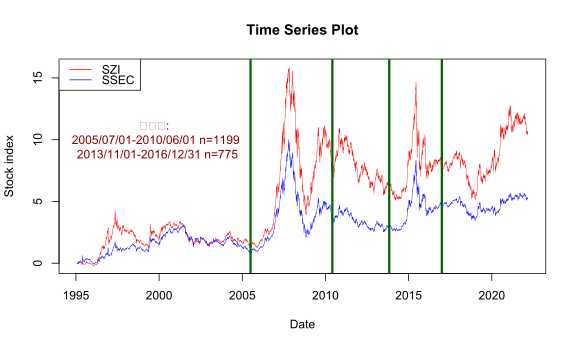
\includegraphics[height = 5.5cm]{fig/Time series w duration.jpg}
    \label{fig:Time slot selection plot}  
  \end{figure}
\end{frame}

\subsection{Exploration Data Analysis}
\begin{frame}{Statistics Characteristics}
  \begin{itemize}
    \item Stock market, interval, N.
    \item Transform to return rate.
    \item Basic statistics.
    \item Characteristic plots.
  \end{itemize}

  % \begin{figure}[htbp]
  %   \centering
  %   \hyperlink{Characteristics}{\begin{minipage}[t]{0.49\columnwidth}
  %     \flushleft
  %     \includegraphics[width=\columnwidth]{fig/Normality_plot.jpg}
  %     % \caption{Dialogue Rounds of Traditional Free Q\&A strategy}
  %     \label{fig:Normality plot} 
  %   \end{minipage}}
  %   \hypertarget{Characteristics plots}{\begin{minipage}[t]{0.49\columnwidth}
  %     \flushright
  %     \includegraphics[width=\columnwidth]{fig/SSEC_05_10.jpg}
  %     % \caption{Result Coverage of Traditional Free Q\&A strategy}
  %     \label{fig:Tirplot} 
  %   \end{minipage}}
  % \end{figure}

  \begin{figure}[htp]
    \centering
    \hypertarget{Leptokurtosis}{\includegraphics[height = 5cm]{fig/Normality_plot.jpg}}
  \end{figure}
\end{frame}


\begin{frame}
  \begin{table}[htbp]
    \centering
    \tiny
      \begin{tabular}{cp{4.315em}ll}
      \toprule
      \multicolumn{4}{c}{\small{\textbf{Basic Statistics for Four Datasets}}} \\
      \midrule
      \multicolumn{2}{c}{} & \multicolumn{1}{p{13.94em}}{SSEC} & \multicolumn{1}{p{13.94em}}{SZI} \\
      \cmidrule{2-4}    \multicolumn{1}{c}{\multirow{6}[12]{*}{2005/07/01-2010/06/01}} & n   & 1199 & 1199 \\
      \cmidrule{2-4}        & min & \multicolumn{1}{p{13.94em}}{      Date   Close    Rate\newline{}2007-02-27 2771.79 -0.093} & \multicolumn{1}{p{13.94em}}{      Date   Close    Rate\newline{}2007-02-27 7790.82 -0.098} \\
      \cmidrule{2-4}        & max & \multicolumn{1}{p{13.94em}}{      Date   Close    Rate\newline{}2008-09-19 2075.09 0.090} & \multicolumn{1}{p{13.94em}}{      Date    Close   Rate\newline{}2008-04-24 12914.76 0.092} \\
      \cmidrule{2-4}        & sd  & 0.02042495 & 0.02245218 \\
      \cmidrule{2-4}        & skewness & -0.434222 & -0.4328163 \\
      \cmidrule{2-4}        & kurtosis & 2.336674 & 1.757114 \\
      \midrule
      \multicolumn{1}{c}{\multirow{6}[12]{*}{2013/11/01-2016/12/31}} & n   & 775 & 775 \\
      \cmidrule{2-4}        & min & \multicolumn{1}{p{13.94em}}{      Date   Close    Rate\newline{}2015-08-24 3209.91 -0.089} & \multicolumn{1}{p{16em}}{      Date    Close   Rate\newline{}2015-06-26 14398.78 -0.086} \\
      \cmidrule{2-4}        & max & \multicolumn{1}{p{13.94em}}{      Date   Close    Rate\newline{}2015-07-09 3709.33 0.056} & \multicolumn{1}{p{13.94em}}{      Date   Close    Rate\newline{}2015-09-16 9890.43 0.063} \\
      \cmidrule{2-4}        & sd  & 0.01740382 & 0.01978073 \\
      \cmidrule{2-4}        & skewness & -1.207604 & -0.9666158 \\
      \cmidrule{2-4}        & kurtosis & 5.448543 & 3.513512 \\
      \bottomrule
      \end{tabular}%
    \label{tab:addlabel}%
  \end{table}%

\end{frame}

\begin{frame}
  \begin{figure}[htp]
    \centering
    \hypertarget{volatility clustered}{\includegraphics[height = 8cm]{fig/SSEC_05_10.jpg}}
      \label{fig:Tirplot} 
  \end{figure}
\end{frame}


\begin{frame}
  \begin{figure}[htp]
    \centering
      \hypertarget{series corr}{\includegraphics[width = .9\columnwidth]{fig/Acf_pacf_plot.png}}
  \end{figure}
\end{frame}


\begin{frame}{Basic Statistical Tests}
  \begin{itemize}
    \item Normality: Normality plot, QQ-plot, kstest, jbtest, swtest.
    \item Unit root: ADF test.
    \item Serial correlation: ACF \& PACF, BDS test($H_o$: $i.i.d.$ sereis.)
    \item ARCH effect: Engle's LM test, McLeod-Li test.
  \end{itemize}
\end{frame}


% 分两列,一列图,一列文字
\subsection{Modelling Methods}
\begin{frame}{Modelling Methods}
  \begin{columns} % 分列
    \column{0.62\textwidth} % 文字列,0.x 倍宽
    \begin{itemize}
      \item Method 1:\\
      \emph{Building a volatility model usually consists five steps:\\
      1.Specify a mean equation.\\
      2.Use the residuals of the mean equation to test for ARCH effects.\\
      3.Specify a volatility model.\\
      4.Perform a joint estimation.\\
      5.Check the fitted model.}\\
      --- Ruey. S. Tsay, Analysis of Financial Time Series
      \item Method 2:\\
      Compare the AIC/BIC among all possible ARMA-GARCH models.
    \end{itemize}
    \column{0.7\textwidth}

    \begin{figure}[htp]
      \flushleft
        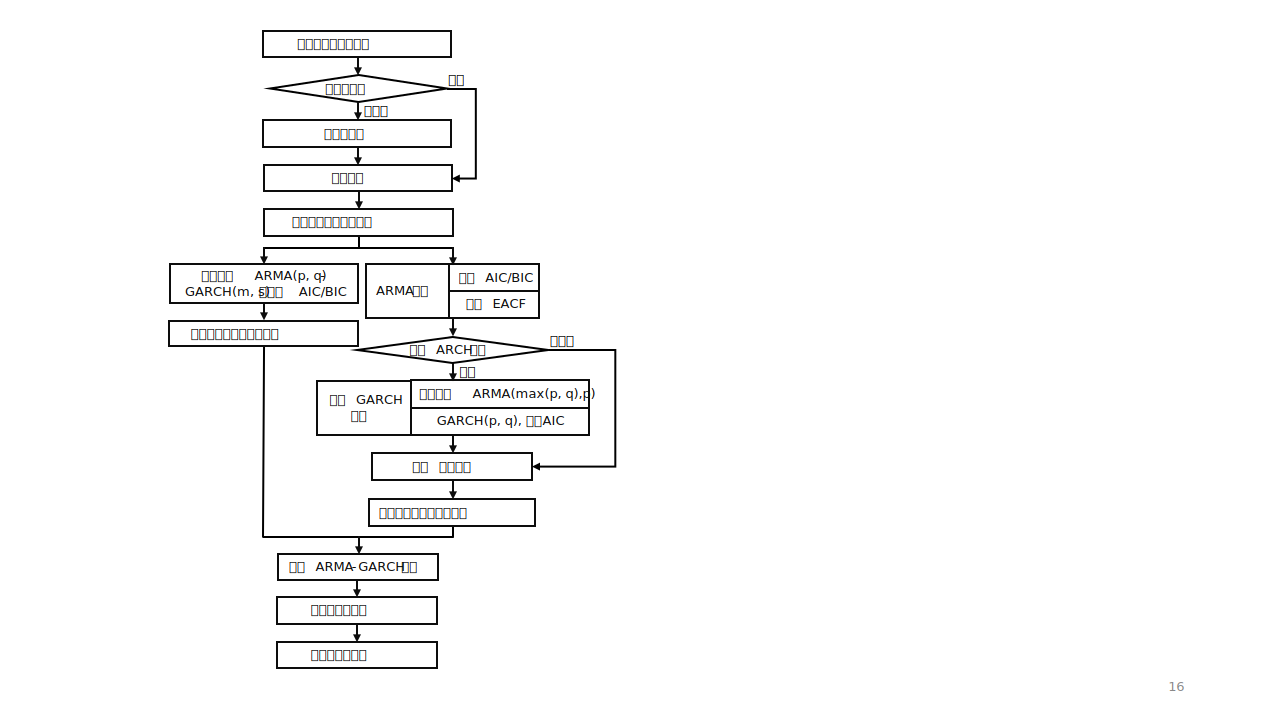
\includegraphics[width = .6\columnwidth]{fig/process.jpg}
        \label{fig:process_plot} 
    \end{figure}
  \end{columns}
\end{frame}

\subsection{Innovation distribution}
\begin{frame}{Innovation distribution}
  As what we mentioned earlier, the finantial time series is leptokurtosis, negative biased and failed to pass the normality tests. Moreover, the adjusted pearson goodness-of-fit test also suggests normal distribution is not good enough.
  \begin{block}{Common used innovation distributions}
    \begin{itemize}
      \item Symmetric distributions: \\
      Normal, Student, GED (generalized error distribution).
      \item Asymmetric distributions: \\
      Skewed normal, Skewed Student, Skewed GED.
    \end{itemize}
  \end{block}
\end{frame}


\begin{frame}{Scope of potential models for model selection}
\begin{table}[htbp]
  \small
    \begin{tabular}{p{16em}p{5em}p{5em}}
    \toprule
    \multicolumn{3}{C{26em}}{\textbf{Scope of potential models for model selection}} \\
    \midrule
    \multicolumn{1}{r}{} & Tsay方法 & 全部回归 \\
    \midrule
    ARMA & √   & √ \\
    \midrule
    GARCH family: including GARCH, IGARCH, TGARCH model & GARCH only   & √ \\
    \midrule
    Innovation distribution: including Normal, Student, GED, Skewed normal, Skewed Student, Skewed GED. & Normal only & √ \\
    \midrule
    Parameter restrictions: Omega=0, mu=0 & √   & √ \\
    \bottomrule
    \end{tabular}%
  \label{tab:addlabel}%
\end{table}%

\end{frame}

\subsection{Conclusion}
\begin{frame}{Conclusion}
  % \begin{table}[htbp]
  %   \tiny
  %   \caption{ARMA-GARCH Model Regression Result}
  %   \centering
  %     \begin{tabular}{rp{2em}p{18em}p{18em}}
  %       \toprule[1pt]
  %       \multicolumn{2}{p{7.375em}}{数据集} & 包含偏分布 & 不包含偏分布 \\
  %       \midrule
  %       \multicolumn{1}{r}{\multirow{2}[2]{*}{050701-100601}} & SSEC & ARMA(2,2)-IGARCH(1,1)-omega=0-SGED & ARMA(2,2)-IGARCH(1,1)-omega=0-GED \\
  %       \cmidrule{2-4}        
  %           & SZI & ARMA(2,2)-IGARCH(1,1)-omega=0-SGED & ARMA(2,2)-IGARCH(1,1)-omega=0-GED  \\
  %       \midrule
  %       \multicolumn{1}{r}{\multirow{2}[2]{*}{131101-161231}} & SSEC & ARMA(2,2)-IGARCH(1,1)-omega=0-mu=0-ar1=0-ma1=0-SGED & ARMA(2,2)-IGARCH(1,1)-omega=0-mu=0-ar1=0-ma1=0-GED \\
  %       \cmidrule{2-4}        
  %           & SZI & ARMA(2,2)-IGARCH(1,1)-omega=0-mu=0-SGED & ARMA(2,2)-IGARCH(1,1)-omega=0-GED \\
  %       \bottomrule[1pt]
  %     \end{tabular}
  % \end{table}

  % Table generated by Excel2LaTeX from sheet 'Sheet1'
\begin{table}[htbp]
  \centering
  \tiny
    \begin{tabular}{rp{2em}p{12em}p{12em}p{8em}p{8em}}
    \toprule
    \multicolumn{2}{c}{\multirow{2}[4]{*}{数据集}} & \multicolumn{2}{C{26em}}{只包含正态分布} & \multirow{2}[4]{*}{不包含偏分布} & \multirow{2}[4]{*}{包含偏分布} \\
\cmidrule{3-4}    \multicolumn{2}{c}{} & \multicolumn{1}{c}{Tsay方法} & \multicolumn{1}{c}{全部回归} & \multicolumn{1}{c}{} & \multicolumn{1}{c}{} \\
    \midrule
    \multicolumn{1}{r}{\multirow{2}[4]{*}{05-10}} & SSEC & ARMA(2,2)-IGARCH(1,1)-omega=0-mu=0-NORM & ARMA(2,2)-IGARCH(1,1)-omega=0-mu=0-NORM & ARMA(2,2)-IGARCH(1,1)-omega=0-GED & ARMA(2,2)-IGARCH(1,1)-omega=0-SGED \\
\cmidrule{2-6}        & SZI & ARMA(2,2)-IGARCH(1,1)-omega=0-mu=0-NORM & ARMA(2,2)-IGARCH(1,1)-omega=0-mu=0-NORM & ARMA(2,2)-IGARCH(1,1)-omega=0-GED  & ARMA(2,2)-IGARCH(1,1)-omega=0-SGED \\
    \midrule
    \multicolumn{1}{r}{\multirow{2}[4]{*}{13-16}} & SSEC & ARMA(2,2)-IGARCH(1,1)-omega=0-mu=0-ar1=0-ma1=0-NORM & ARMA(2,2)-IGARCH(1,1)-omega=0-mu=0-ar1=0-ma1=0-NORM & ARMA(2,2)-IGARCH(1,1)-omega=0-mu=0-ar1=0-ma1=0-GED & ARMA(2,2)-IGARCH(1,1)-omega=0-mu=0-ar1=0-ma1=0-SGED \\
\cmidrule{2-6}        & SZI & ARMA(2,2)-IGARCH(1,1)-omega=0-mu=0-NORM & ARMA(2,2)-IGARCH(1,1)-omega=0-mu=0-NORM & ARMA(2,2)-IGARCH(1,1)-omega=0-GED & ARMA(2,2)-IGARCH(1,1)-omega=0-mu=0-SGED \\
    \bottomrule
    \end{tabular}%
  \label{tab:addlabel}%
\end{table}%

  \tiny
  \begin{itemize}
    \item With skewed distribution, the SGED is optimal among all datasets. 
    \item Without skewed distribution, the GED is the optimal one.
    \item Generally, the optimal model is ARMA(2,2)-IGARCH(1,1)-omega=0.  
    \item The \hypertarget{TGARCH back}{\hyperlink{TGARCH}{TGARCH}} model is not significant among all datasets.
    \item Mu is not significant under normal innovation distribution, but significant under GED innovation distribution.
  \end{itemize}
\end{frame}


\subsection{Residuals Analysis}
\begin{frame}{Residuals Analysis}
  \begin{itemize}
    \item QQ-plot
    \item Serieial correlation: ACF \& PACF, BDS test
    \item Prediction
  \end{itemize}

  \begin{figure}[bp]
    \centering
    \begin{minipage}[t]{0.53\columnwidth}
      \flushleft
      \includegraphics[width=1\columnwidth]{fig/Rolling forecast.png}
      \label{fig:Rolling forecast plot} 
    \end{minipage}
    \begin{minipage}[t]{0.45\columnwidth}
      \flushright
      \includegraphics[width=\columnwidth]{fig/ged-qq-plot.png}
      \label{fig:ged qq plot} 
    \end{minipage}
  \end{figure}
\end{frame}


\begin{frame}{Residuals Analysis}
  \begin{figure}[htp]
    \centering
    \includegraphics[width = \columnwidth]{fig/res acf pacf plot.png}
    \label{fig:res plot}
  \end{figure}
\end{frame}


\subsection{Discussions}
\begin{frame}{Discussion}
  \begin{block}{Discussion 1: Robustness of two model selection methods}
    \begin{table}[htbp]
      \begin{threeparttable}
        \centering
        \tiny
        \begin{tabular}{cp{2em}C{5.94em}C{5.94em}C{9.065em}C{9.065em}}
          \toprule
          \multicolumn{6}{c}{\footnotesize{\textbf{两种模型选择方法在Normal innovation假设下的结果比较}}} \\
          \midrule
          \multicolumn{2}{c}{\multirow{2}[4]{*}{数据集}} & \multicolumn{2}{p{11.88em}}{Compare among all possible models} & \multicolumn{2}{p{18.13em}}{Tsay's method} \\
          \cmidrule{3-6}    \multicolumn{2}{c}{} & \multicolumn{1}{c}{ARMA} & \multicolumn{1}{c}{GARCH} & \multicolumn{1}{c}{ARMA} & \multicolumn{1}{c}{GARCH} \\
          \cmidrule{1-6}    \multicolumn{1}{c}{\multirow{2}[4]{*}{050701-100601}} & SSEC & (2, 2) & (1, 1) & (2, 2) & (1, 1) \\
          \cmidrule{2-6}        & SZI & (2, 2) & (1, 1) & (2, 2) & (1, 1) \\
          \midrule
          \multicolumn{1}{c}{\multirow{2}[4]{*}{131101-161231}} & SSEC & (2, 2) & (1, 1) &  EACF/AIC提示过大的模型,BIC提示(2, 2) & (1, 1) \\
          \cmidrule{2-6}        & SZI & (2, 2) & (1, 1) &  EACF/AIC提示过大的模型,BIC提示(3, 2) &  EACF/AIC提示过大的模型,BIC提示ARMA(3, 2) 即(3, 2) $^{\textbf{a}}$\\
          \bottomrule
        \end{tabular}

        % 表格尾注
        \begin{tablenotes}
          %\footnotesize   %% If you want them smaller like foot notes
          \item[a] Note: 在Joint estimation中,一些参数不显著,消去之后得到\textbf{ARMA(2,2)-GARCH(1,1)}模型。
        \end{tablenotes}
      \end{threeparttable}
    \end{table}
  \end{block}
\end{frame}

\begin{frame}{Discussion}
  \begin{block}{Discussion 1: Robustness of two model selection methods}
    回顾: 2015年后半年打击融资融券交易:\\
    \begin{itemize}
      \item 总体来看融资融券交易还是可以有效地平抑市场波动。\\
      \begin{flushright}
        ——《融资融券对中国股票市场波动影响的研究》江西财经大学
      \end{flushright}
      \item 深圳市场受两融交易的影响比上海市场更大。\\
      \begin{flushright}
        ——《融资融券对中国A股市场波动的影响—基于事件研究法下沪深两市的比较研究》\\
      \end{flushright}
      提示: 深圳市场受两融交易限制,救市政策影响,熔断政策影响较大,市场发生超出正常运行的波动,Tsay方法鲁棒性不足,估计出现较大偏差。
    \end{itemize}
  \end{block}
		The ARCH model only takes finite past realizations into consideration, thus its memory is not long enough, which result in a larger parameters. Bollerslev(1986) proposed a strong extension known as the generalized ARCH model. The introduction of past conditional variance dramatically eliminates the parameters. For most economic situations, a GARCH(1,1) model is enough. 
\end{frame}

\begin{frame}{Discussion}
  \footnotesize
  \begin{block}{Discussion 2: TGARCH Not Significant}
    其次,从表2-7和表2-8中我们可以看出EGARCH(1,1)模型和GJR-GARCH(1,1)模型中\textcolor{red}{用来刻画波动不对称性的参数均不显著},这说明在所研究时间段中上证180指数的波动并不存在明显的杠杆效应,这与我们最常接触的假定条件是有所出入的。在此笔者推断\textcolor{red}{可能是由于本次选取的样本数据跨越时间较长,且包含了一段完整的牛市熊市的转换,不同市场状态的转换可能会一定程度上抵消波动的不对称特征,从而使得对于整体波动特征的研究呈现出杠杆效应不显著的结果。}另外还可能是由于本论文选择的样本数据是成分指数上证180收益率序列,其中包含的样本均是规模大、行业代表性强的公司股票,受内部负面消息及外部冲击的影响程度相对较小。同时随着投资知识的不断普及,投资者在进行投资行为时也逐渐趋于理性,从而使得上海股票市场的不对称效应没有之前那样显著。
    \begin{flushright}
      ---《基于GARCH模型的上证180指数收益率波动研究》中南财经政法大学 
    \end{flushright}

    还有可能是由于我国股票市场受政策影响较大,在大的下跌之后可能伴随着救市政策带来的大的上涨,从而在一定程度上抵消了市场的不对称性。\vskip 0.3cm 

    以上,我们虽然能够观察到收益率序列的负偏态,但是无法捕捉到显著的不对称性。提示我们: 更换收益率数据, 讨论描述不对称性的模型的有效性。
  \end{block}
\end{frame}

\begin{frame}{Discussion}
  \begin{block}{Discussion 3: Further Research}
    \begin{itemize}
      \item 更换数据时间段,区分牛市,熊市,盘整期进行研究,寻找TGARCH效应。\\
      \item 更换高频数据(10min数据)。\\
      \item 拓展两个讨论,即: 讨论两种估计方法; 讨论15年股灾对Tsay估计方法的影响。
    \end{itemize}
  \end{block}
\end{frame}

% \begin{frame}
%   \begin{block}
%     \begin{itemize}
%       \item 更换数据时间段,区分牛市,熊市,盘整期进行研究,寻找TGARCH效应。\\
%       \item 更换高频数据(10min数据)。\\
%       \item 拓展两个讨论,即: 讨论两种估计方法; 讨论15年股灾对Tsay估计方法的影响。
%     \end{itemize}
%   \end{block}
% \end{frame}

\end{document}